\documentclass[11pt,aspectratio=169]{beamer}
\usepackage[utf8]{inputenc}
\usepackage[T1]{fontenc}
\usepackage{lmodern}
\usepackage[ngerman]{babel}
\usepackage{tikz}
\usetheme{Hannover}

\begin{document}
	\author{Joshua Bär und Michael Steiner}
	\title{Reed-Solomon-Code}
	\subtitle{}
	\logo{}
	\institute{OST Ostschweizer Fachhochschule}
	\date{26.04.2021}
	\subject{Mathematisches Seminar}
	\setbeamercovered{transparent}
	\setbeamertemplate{navigation symbols}{}
	\begin{frame}[plain]
		\maketitle
	\end{frame}
	\section{Introduction}
	\begin{frame}
		\frametitle{Idee}
		
	\end{frame}

	\begin{frame}
		\begin{figure}
			\only<1>{
			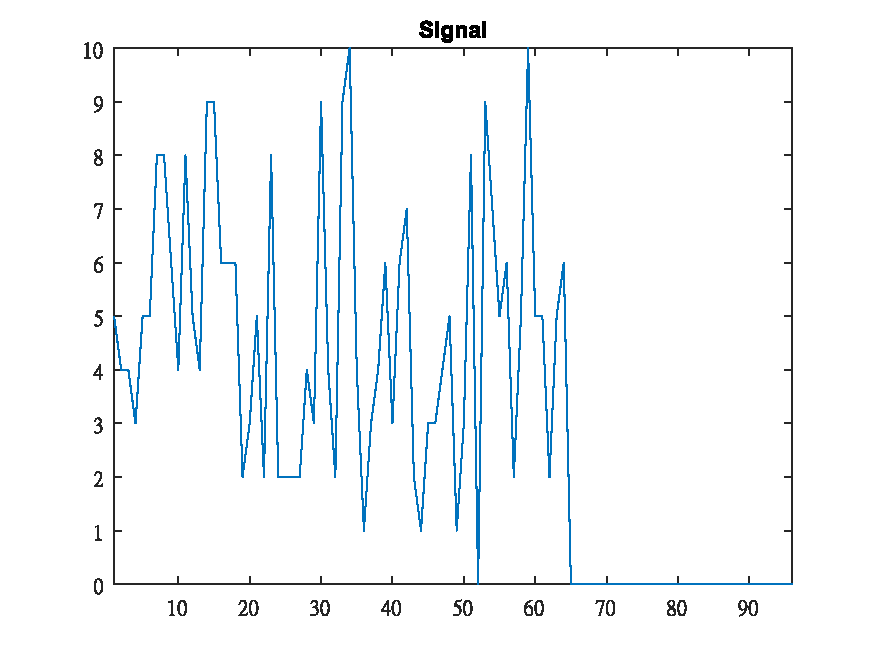
\includegraphics[width=0.9\linewidth]{images/fig1.pdf}
			}
			\only<2>{
			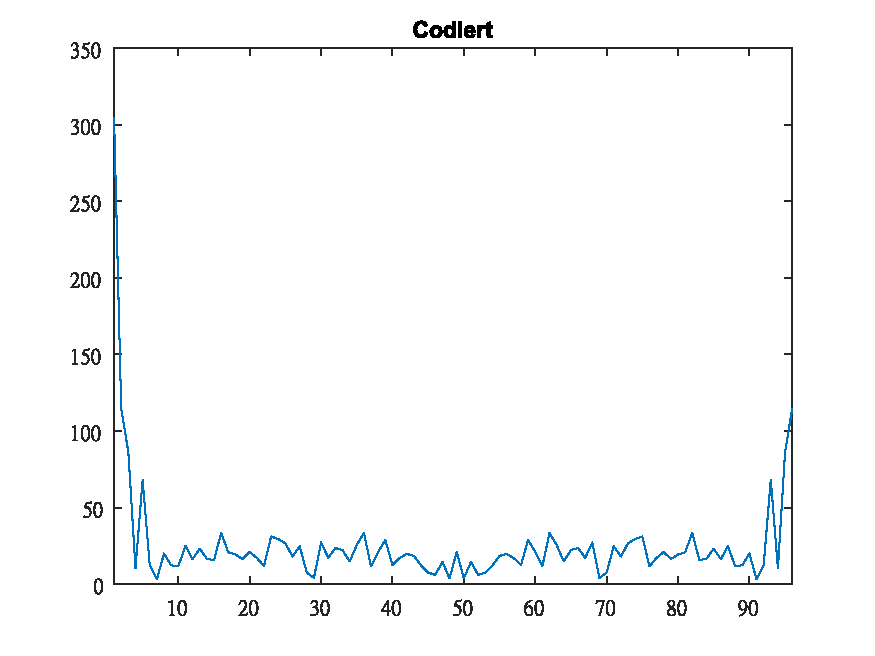
\includegraphics[width=0.9\linewidth]{images/fig2.pdf}
			}
			\only<3>{
			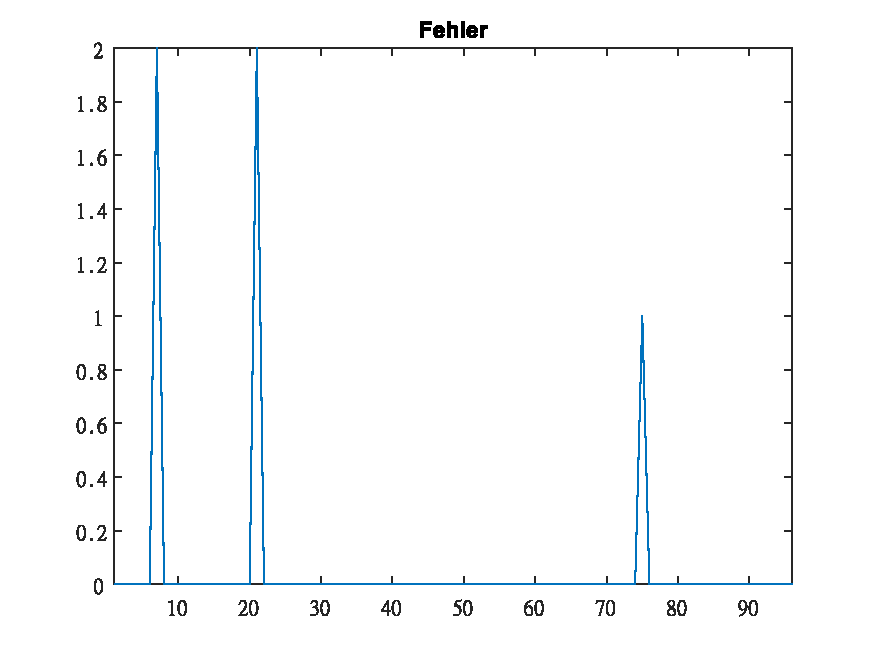
\includegraphics[width=0.9\linewidth]{images/fig3.pdf}
			}
			\only<4>{
			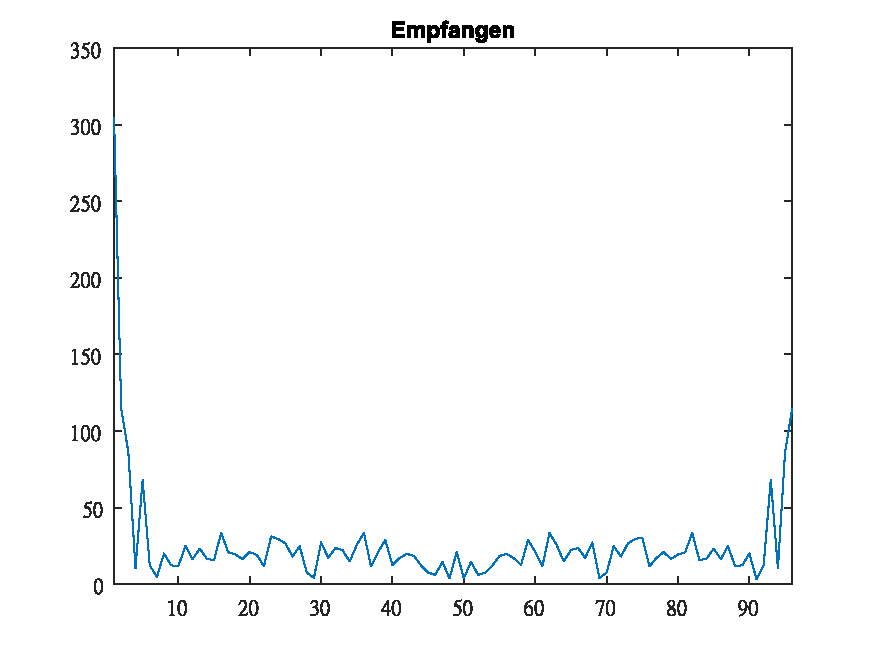
\includegraphics[width=0.9\linewidth]{images/fig4.pdf}
			}
			\only<5>{
			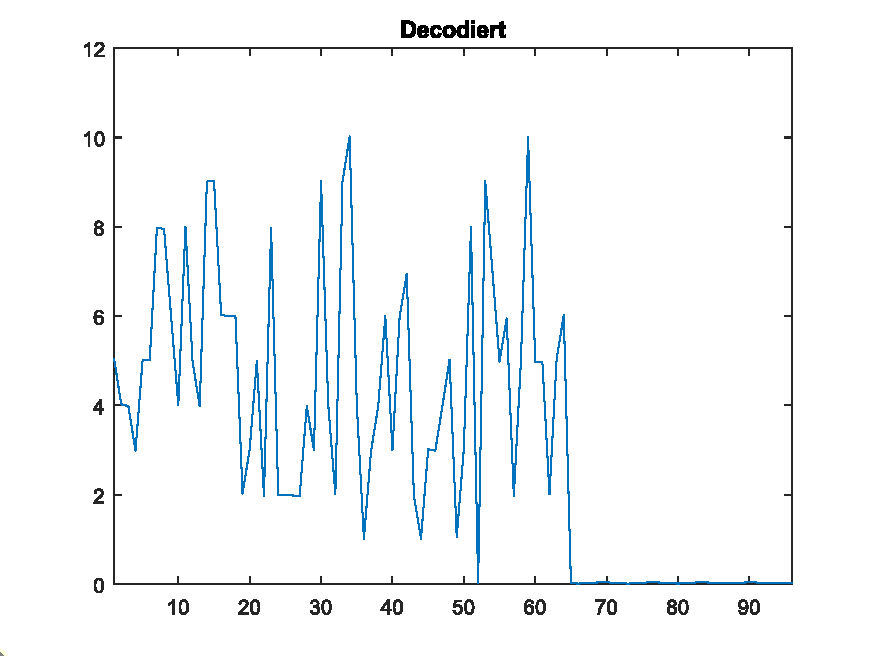
\includegraphics[width=0.9\linewidth]{images/fig5.pdf}
			}
			\only<6>{
			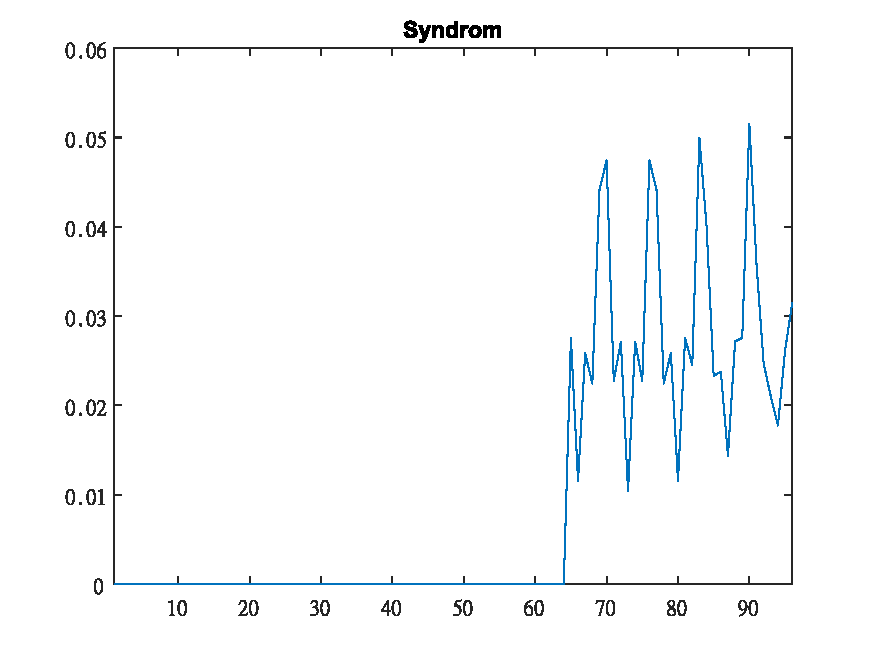
\includegraphics[width=0.9\linewidth]{images/fig6.pdf}
			}
			\only<7>{
			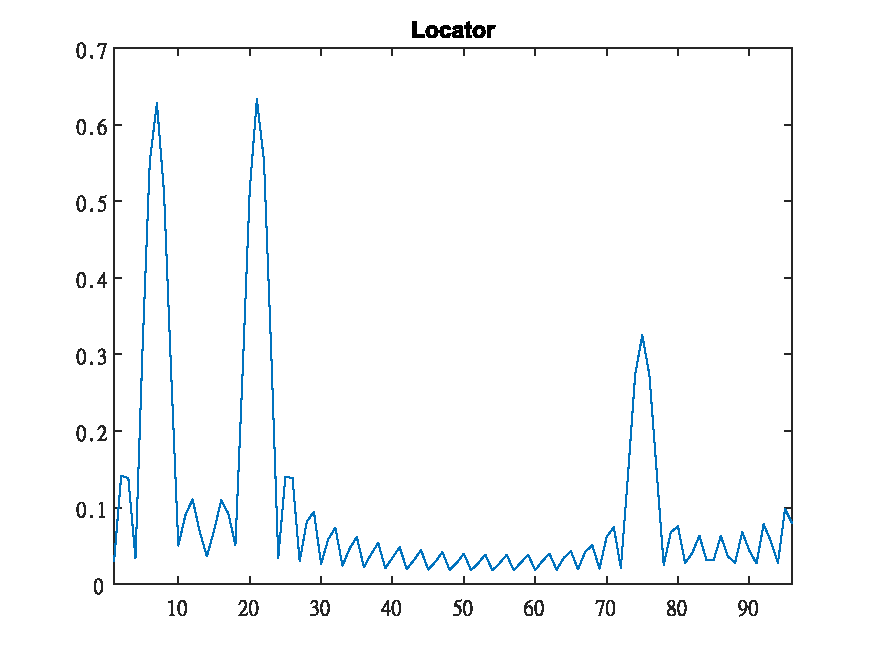
\includegraphics[width=0.9\linewidth]{images/fig7.pdf}
			}
	\end{figure}
	\end{frame}

	\begin{frame}
		Übertragen von den Zahlen 
		\textcolor{blue}{2}, \textcolor{blue}{1}, \textcolor{blue}{5} 
		als $ p(x) = \textcolor{blue}{2}x^2 + \textcolor{blue}{1}x + \textcolor{blue}{5} $.\newline
		Versende $ (p(1),p(2),...,p(7)) = (\textcolor{green}{8}, 
			\textcolor{green}{15}, \textcolor{green}{26},
			\textcolor{green}{ 41}, \textcolor{green}{60}, 
			\textcolor{green}{83}, \textcolor{green}{110})$
		\only<1>{
		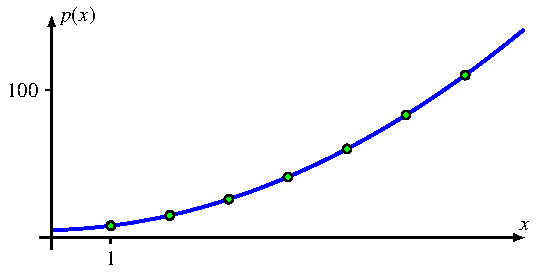
\includegraphics[]{images/polynom1.pdf}}
		\only<2>{
		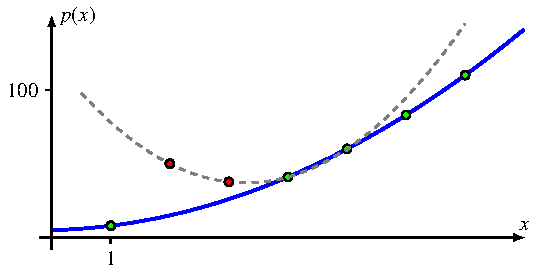
\includegraphics[]{images/polynom2.pdf}}
	\end{frame}

	
\end{document}